%%%%%%%%%%%%%%%%%%%%%%%%%%%%%%%%%%%%%%%%%
% Stylish Article
% LaTeX Template
% Version 2.2 (2020-10-22)
%
% This template has been downloaded from:
% http://www.LaTeXTemplates.com
%
% Original author:
% Mathias Legrand (legrand.mathias@gmail.com) 
% With extensive modifications by:
% Vel (vel@latextemplates.com)
%
% License:
% CC BY-NC-SA 3.0 (http://creativecommons.org/licenses/by-nc-sa/3.0/)
%
%%%%%%%%%%%%%%%%%%%%%%%%%%%%%%%%%%%%%%%%%

%----------------------------------------------------------------------------------------
%	PACKAGES AND OTHER DOCUMENT CONFIGURATIONS
%----------------------------------------------------------------------------------------

\documentclass[fleqn,10pt]{SelfArx} % Document font size and equations flushed left

\usepackage[polish]{babel} % Specify a different language here - english by default
\usepackage[utf8]{inputenc} 	% W celu dekodowania polskich znaków
\usepackage[T1]{fontenc}
%\usepackage{polski}

\usepackage[bottom]{footmisc}	% Używamy, by stopka zawsze była na samym dole strony
\usepackage{changepage}			% dla customowych marginesów

\usepackage{listings}
\usepackage[most]{tcolorbox}
\usepackage{inconsolata}

\newtcblisting[auto counter]{sexylisting}[2][]{sharp corners, 
    fonttitle=\bfseries, colframe=airforceblue, listing only, 
    listing options={basicstyle=\small\ttfamily,language=C++, numbers=left, 
					numberstyle=\scriptsize,   
    				xleftmargin=0.6em},
    title=Listing \thetcbcounter: #2, #1}

\usepackage{graphicx} % Required for including images
\graphicspath{{Figures/}{./}} % Specifies where to look for included images (trailing slash required)

\usepackage{float} % Allows more precisely positioning floats e.g. \begin{figure}[H]

\usepackage{lipsum} % Required to insert dummy text. To be removed otherwise

%----------------------------------------------------------------------------------------
%	COLUMNS
%----------------------------------------------------------------------------------------

\setlength{\columnsep}{0.55cm} % Distance between the two columns of text
\setlength{\fboxrule}{0.75pt} % Width of the border around the abstract

%----------------------------------------------------------------------------------------
%	COLORS
%----------------------------------------------------------------------------------------

\definecolor{color1}{RGB}{0,0,90} % Color of the article title and sections
\definecolor{color2}{RGB}{0,20,20} % Color of the boxes behind the abstract and headings

\definecolor{airforceblue}{rgb}{0.36, 0.54, 0.66}

%----------------------------------------------------------------------------------------
%	HYPERLINKS
%----------------------------------------------------------------------------------------

\usepackage{hyperref} % Required for hyperlinks

\hypersetup{
	hidelinks,
	colorlinks,
	breaklinks=true,
	urlcolor=color2,
	citecolor=color1,
	linkcolor=color1,
	bookmarksopen=false,
	pdftitle={Title},
	pdfauthor={Author},
}

%----------------------------------------------------------------------------------------
%	ARTICLE INFORMATION
%----------------------------------------------------------------------------------------

\JournalInfo{Politechnika Poznańska, Poznań, \today} % Journal information
\Archive{Artykuł przeglądowy} % Additional notes (e.g. copyright, DOI, review/research article)

\PaperTitle{Przegląd ezoterycznych języków programowania} % Article title

\Authors{Mateusz Szuda\textsuperscript{1}} % Authors
\affiliation{\textsuperscript{1}\textit{student 3 roku Teleinformatyki, nr indeksu 144379, Politechnika Poznańska}} % Author affiliation

\Keywords{ezoteryczne --- języki --- programowania} % Keywords - if you don't want any simply remove all the text between the curly brackets
\newcommand{\keywordname}{Słowa kluczowe} % Defines the keywords heading name

%----------------------------------------------------------------------------------------
%	ABSTRACT - streszczenie
%----------------------------------------------------------------------------------------

\Abstract{
	Istnieje pewna grupa języków programowania zwana językami ezoterycznymi (ang. \textbf{\textit{esolang}}). \textit{Są one tworzone w celu badania i demonstracji niekonwencjonalnych technik programistycznych oraz metod programowania.
	Nie są one natomiast przeznaczone do pisania rzeczywistych aplikacji.}\cite{Wiki:EsotericPL}
	Ich twórcy skupiają się na dążeniu do stworzenia języka \textit{dziwnego} - \textbf{Malbolge}, \textit{minimalistycznego} - \textbf{Brainfuck}, \textit{o danym motywie} - \textbf{Shakespeare}, czy stworzonego dla \textit{zwykłego żartu} - \textbf{Ook!}.
	Zostało przedstawione tylko kilka przykładów języków oraz ich zastosowania, a w dalszej części artykułu poruszę kwestie związane z ich genezą,
	opiszę wymienione języki oraz zagłębię się w temat celów, jakimi kierowali się programiści podczas ich tworzenia. 
	Dodatkowo przedstawię semantykę tych języków okraszoną przykładowymi programami napisanymi za ich pomocą.
}

%----------------------------------------------------------------------------------------

\begin{document}

\maketitle % Output the title and abstract box

\tableofcontents % Output the contents section

\thispagestyle{empty} % Removes page numbering from the first page

%----------------------------------------------------------------------------------------
%	ARTICLE CONTENTS
%----------------------------------------------------------------------------------------

\section*{Wstęp} % The \section*{} command stops section numbering

\addcontentsline{toc}{section}{Wstęp} % Adds this section to the table of contents
	Opisując pojęcie \textit{języka programowania}, większość osób wyobraża sobie je jako narzędzie,
	zbiór zasad określających dane działania. Kod taki jest następnie kompilowany \textit{(np. C, C++)}, 
	bądź interpretowany \textit{(np. Python)} przez komputer, który wykonuje określone instrukcje zawarte w kodzie.
	Jednymi z najbardziej popularnych języków pozwalających nam na takie działania są: \underline{Python, Java, C, C++, JavaScript,} \underline{C\#, R, Go} 
	\cite{IEEESpectrum:popularLang2021}\footnote{wybór 8 najbardziej popularnych języków programowania w 2021 roku według serwisu IEEE spectrum:
		\url{https://spectrum.ieee.org/top-programming-languages-2021}}.
	Są to języki proste w swoim użyciu, zawierające bogatą i szeroko opisaną składnię językową. 
	Nie każdy język natomiast nadaje się do przetwarzania pewnych problemów, z którymi mierzą się programiści. 
	Program napisany w jednym języku może się wykonywać szybciej niż w drugim. To samo tyczy się objętości samych programów, 
	ich kompilatorów, czy samego kodu źródłowego. Dodatkowo należy mieć też na uwadze fakt, 
	iż jedne języki programowania są bardziej odpowiednie do rozwiązywania określonych zadań, konkretnych problemów, 
	w porównaniu do innych tworów.
	\indent Dobrym przykładem byłoby tutaj przywołanie grupy języków R, SQL i Matlab w opozycji do C, C++ i Javy. 
	Pierwsza grupa to języki przeznaczenia specjalistycznego, wykorzystywane do wszelakich obliczeń statystycznych, 
	czy algorytmicznych, reprezentacji graficznej wyników, czy wykonywania operacji bazodanowych. 
	Druga grupa są to języki ogólnego przeznaczenia, które pozwalają na stworzenie wysokowydajnych aplikacji, istniejące od wielu lat. 
	Ich niewątpliwą zaletą jest również fakt istnienia ogromnej bazy dokumentacji oraz aplikacji napisanych za pomocą tych języków. 
	\textit{W rzeczy samej, nawet znacząca część języka Python, jak i jego dokumentacji jest napisana w języku C z powodów wydajnościowych}
	\cite{IEEESpectrum:popularLang2021}\footnote{„Indeed, significant parts of Python itself and its libraries are written in C for performance reasons.” ~ \url{https://spectrum.ieee.org/top-programming-languages-2021}}.

%------------------------------------------------

\section{Czas na języki ezoteryczne}
\subsection{Pojęcie języka ezoterycznego}
	W przeciwieństwie do języków programowania tworzonych w celu produktywnego i efektywnego
	projektowania i budowania aplikacji, \textbf{języki ezoteryczne} tworzone są w innych celach: Mogą one reprezentować pewne idee \textbf{proof-of-concept},
	demonstrować \textbf{minimalizację} składni języka, który będzie nadal używalny, zachowując jednocześnie \textbf{uniwersalność}.
	Mogą one pomóc w udowodnieniu pewnych konceptów matematycznych, czy ustaleniu granic analiz złożoności.
	Proces projektowania języków ezoterycznych można zdefiniować jako operacja artystyczna,
	będąca wynikiem, a wręcz ekspresją ludzkiego intelektu, dowcipu, czy zmysłu \textcolor{red}{estetyki}.
	Mogą być również stworzone w celu podjęcia się swego rodzaju rywalizacji między programistami, bądź wyzwania, czy to dla siebie, czy dla hipotetycznego użytkownika.
	Istnieje jeszcze kolejna grupa języków ezoterycznych - języki prześmiewcze, napisanych ku uciesze autorów, użytkowników, czy choćby czytelników ich specyfikacji.\cite{morr2015esoteric}
	Wszystkie wymienione właściwości, jak i charakterystyki języków ezoterycznych wywołują chęć przyjrzenia się im dokładniej oraz poznania zamiarów ekscentrycznych programistów stojących za ich powstaniem.

%------------------------------------------------
% TODO: GENEZA języków eso...

\subsection{Geneza powstania języków ezoterycznych}
Za najstarszy znany język ezoteryczny uważa się \hypertarget{oldestLang}{\textbf{\textit{INTERCAL}}} stworzony w \textbf{1972} roku 
przez \underline{Donalda R. Woodsa} oraz \underline{Jamesa M. Lyona}.

\subsubsection{Prehistoria języków ezoterycznych}
W historii informatyki można natomiast doszukać się informacji o językach, 
które miały wspólną genezę ze współczesnymi językami
ezoterycznymi. Co natomiast odróżniało je od nowoczesnych post-INTERCAL'owych języków ezoterycznych, 
tworzone one były w celach profesjonalnych i całkowicie użytkowych.
Przypatrzmy się przykładowo językowi \textbf{\textit{EXPLOR}}: 
\begin{adjustwidth}{1cm}{0cm}
	Jego główna idea polegała na wykonywaniu się kodu czysto probabilistycznie - każda poszczególna instrukcja ma pewne \textit{prawdopodobieństwo}, 
	które definiuje częstość jej wykonania. W dodatku podczas pisania kodu za jego pomocą nie ma możliwości użycia
	\textit{zmiennych} - każda instrukcja bazuje na aktualnej wartości stanu wyświetlacza, bądź na innych instrukcjach.
	\\\textcolor{green}{(!) Ciekawostka:} języka tego używało wielu artystów, by móc generować obrazy używane do animacji swoich ekspresji, 
	jak i również był nawet używany przez pewien czas jako narzędzie do nauki \textsc{grafiki komputerowej} zarówno artystów, jak i dzieci.
\end{adjustwidth}
Przykładowy program napisany w języku EXPLOR wygląda tak:
\begin{sexylisting}{EXPLOR code}
  dim    (1,1)    (512,384)
  wbt    (1,1)    (abc,012,)
  bxl    (1,1)    40(20,20,45,45,10,10,50,38)1(a.)
ax axl   (1,1)    4,news,01,1(.01)
  axl    (1,1)    4,news,12,1(.12)
  axl    (1,1)    4,news,ab,1(.ab)
  axl    (1,1)    4,news,bc,1(.bc)
  xl     (1,1)    1(.012abac0)
  camera (1,1)    1
cm goto  (x,29,1) ax
\end{sexylisting}
	Według reguł języka, składnia instrukcji wygląda następująco:
	\begin{center}
		\textsc{instrukcja prawdopodobieństwo argumenty}
	\end{center}
\begin{figure}[H] % [H] forces the figure to be placed exactly where it appears in the text
	\centering % Horizontally center the figure
	
\includegraphics[width=0.45\textwidth]{Figures/Explor_example.png} % Include the figure
	\caption{Obraz wygenerowany za pomocą przykładowego kodu zaprezentowanego na \textsc{listingu 1}}
\end{figure}

\subsubsection{Prehistoria języków ezoterycznych - cellular automata}
Do języków ezoterycznych zaliczany jest również dział tzw. \textbf{\textit{automatów komórkowych}}.
Mogą być one uznawane za swego rodzaju języki ezoteryczne, a przynajmniej w sensie ogólnym, jakim określamy całą tematyczną grupę.
Wiele konstruktów określanych jako \textit{automaty komórkowe} jest jednocześnie nazywanymi ezoterycznymi.
Oznacza to nic innego jak fakt, iż mogą one (w teorii) rozwiązyć wszelakie (możliwe do rozwiązania) 
operacje i problemy matematyczne, między innymi \textit{wyliczanie liczby pi} i tak dalej. 
W związku z tym mogą być one uznawane za \textbf{\underline{zupełne} \underline{w sensie Turinga}}.
\begin{adjustwidth}{1cm}{0cm} 
	$\hookrightarrow$ Dowolny zestaw reguł i obiektów, który może być użyty do symulacji \textbf{\textit{Uniwersalnej Maszyny Turinga}}
	jest uważany za \textit{kompletny w sensie Turinga}. Wszystkie modele zupełne w sensie Turinga są sobie tożsame, 
	w takim sensie, że korzystają one z tego samego zestawu funkcji do wyliczeń.\cite{IEEEXplore:TuringCompletnessCivilization}
\end{adjustwidth}
Dzięki takiemu założeniu możemy przyjąć, że automaty: stworzony na początku lat 1950 - opublikowany w \textbf{1966} roku \underline{"29-cio stanowy} \underline{automat" Von Neumanna}
oraz opublikowana w \textbf{1970} roku \underline{"Gra w życie" Johna Conwaya} są jednocześnie jednymi z pierwszych \textbf{\textit{prehistorycznych języków ezoterycznych}}!


%%%%%%%%%%%%%%%%%%%%%%%%%%%%%%%%%%%%%%%%%
% new section - może coś w stylu - OPIS RODZAJÓW wraz z przykładami - te języki, które są najpopularniejsze etc.
% TODO: opisać INTERCAL

\section{Rodzaje języków ezoterycznych \cite{esolangWiki:esolangs}}	%rodzaje celów (proste, joke, niemożliwe do pisania etc.)
										% + podczas Befunge opisać rodzaj języków Funge.

Istnieje wiele powodów przemawiających za stworzeniem języka ezoterycznego.
Wiadomym już jest, że najważniejszą ich właściwością, odróżniającą je od zwykłych języków,
jest fakt, iż nie są one przeznaczone do poważnego, profesjonalnego użytkowania i funckjonowania.
Możemy natomiast wyróżnić kilka głównych przyczyn, którymi kierują się autorzy w trakcie ich konstruowania.
Wiele języków zostanie tutaj wymienionych, a te \underline{podkreślone} zostaną w późniejszej części pracy dogłębniej wytłumaczone:
\begin{itemize}
	\item \textbf{Minimalizm} - popularnym wyborem podczas projektowania danego języka jest stworzenie zestawu jak najmniejszej liczby instrukcji - 
	uproszczone w pewnych aspektach do granic możliwości.
	Języki tego rodzaju, jeśli są \textit{Turing-zupełne}, określane są mianem \textit{grzęzawiska Turinga}:
	"Strzeżcie się grzęzawiska Turinga, w którym wszystko jest możliwe, ale nic nie jest łatwe"\cite{perlisAlan:epigrams}
	Do minimalistycznych języków zaliczyć można \underline{\textbf{brainfuck}}, \textbf{OISC} oraz \textbf{Lazy K}.
	\item \textbf{Nowe koncepty} - wśród języków ezoterycznych bardzo popularnym podejściem w trakcie ich projektowania jest 
	wynajdowanie nowych, alternatywnych sposobów na reprezentację kodu. Dobrymi przykładami tego rodzaju języków są \underline{\textbf{Befunge}}, \textbf{Thue} oraz \textbf{Unlambda}.
	\item \textbf{Dziwność} - niektóre języki tworzone są po to, by uzyskać twór dziwny i trudny do pisania w nim kodu.
	Sztandarowym przykładem byłby tutaj język, uznawany za pionerski wśród języków ezoterycznych - \hyperlink{oldestLang}{\underline{\textbf{INTERCAL}}} - stworzony głównie z powodu,
	by być tak inny jak to możliwe od "normalnych" języków programowania, mimo wielu podobieństw między nim, a konwencjonalnymi językami.
	Drugim bardzo interesującym przypadkiem jest \underline{\textbf{Malbolge}}, który został stworzony po to, by być niemal niemożliwym do użytkowania.
	\item \textbf{Tematyczność} - są to języki bazujące na pewnym, wybranym przez twórcę temacie, niezwiązanym z informatyką.
	Mogą być to języki takie jak \textbf{var'aq} - bazujący na fikcyjnym języku Klingońskim; \underline{\textbf{Shakespeare}} - pisany w formie utworów scenicznych tytułowego angielskiego pisarza;
	oraz \underline{\textbf{Chef}}, którego kod wygląda jak przepisy kulinarne!
	\item \textbf{Zwięzłość} - wiele języków dąży do spełnenia pojęcia "im mniej kodu, tym lepiej". Tego rodzaju języki znane są jako \textit{Golfing languages} i bardzo często używane
	są w konkurencji \textbf{code golf}, której celem jest rozwiązanie danych problemów programistycznych za pomocą jak najmniejszej liczby znaków/bajtów, jak to jest możliwe.
	Kategoria ta obfituje w takie języki jak \textbf{CJam}, \textbf{Pyth}, czy \textbf{GolfScript}.
	\item \textbf{Dowcip} - języki tworzone typowo dla swego rodzaju żartu. Tym niemniej, wiele z nich jest zupełnie funkcjonalnych w celach programistycznych.
	Są to między innymi \textbf{l33k}, \underline{\textbf{Ook!}}, jak i również oba wywodzące się z \textit{brainfuck'a} \underline{\textbf{Moanfuck}} i \underline{\textbf{Fuckfuck}}.
	\item \textbf{Nieczytelność} - zaprojektowane w taki sposób, by odczytywanie kodu było w jak największym stopniu utrudnione, w przeciwieństwie do bycia ciężkimi do pisania, czy zrozumienia.
	Doskonałym przykładem jest tutaj tytułowy \underline{\textbf{Unreadable}}. Bardzo ciekawym przypadkiem jest również wpisujący się w te ramy \underline{\textbf{Whitespace}}.
\end{itemize}

%%%%%%%%%%%%%%%%%%%%%%%%%%%%%%%%%%%%%%%%%

\section{Methods}

\begin{figure*}[ht]\centering % Using \begin{figure*} makes the figure take up the entire width of the page
	
\includegraphics[width=\linewidth]{view}
	\caption{Wide Picture}
	\label{fig:view}
\end{figure*}

\lipsum[4] % Dummy text

\begin{equation}
	\cos^3 \theta =\frac{1}{4}\cos\theta+\frac{3}{4}\cos 3\theta
	\label{eq:refname2}
\end{equation}

\lipsum[5] % Dummy text

\begin{enumerate}[noitemsep] % [noitemsep] removes whitespace between the items for a compact look
	\item First item in a list
	\item Second item in a list
	\item Third item in a list
\end{enumerate}

\subsection{Subsection}

\lipsum[6] % Dummy text

\paragraph{Paragraph} \lipsum[7] % Dummy text
\paragraph{Paragraph} \lipsum[8] % Dummy text

\subsection{Subsection}

\lipsum[9] % Dummy text

\begin{figure}[ht]\centering
	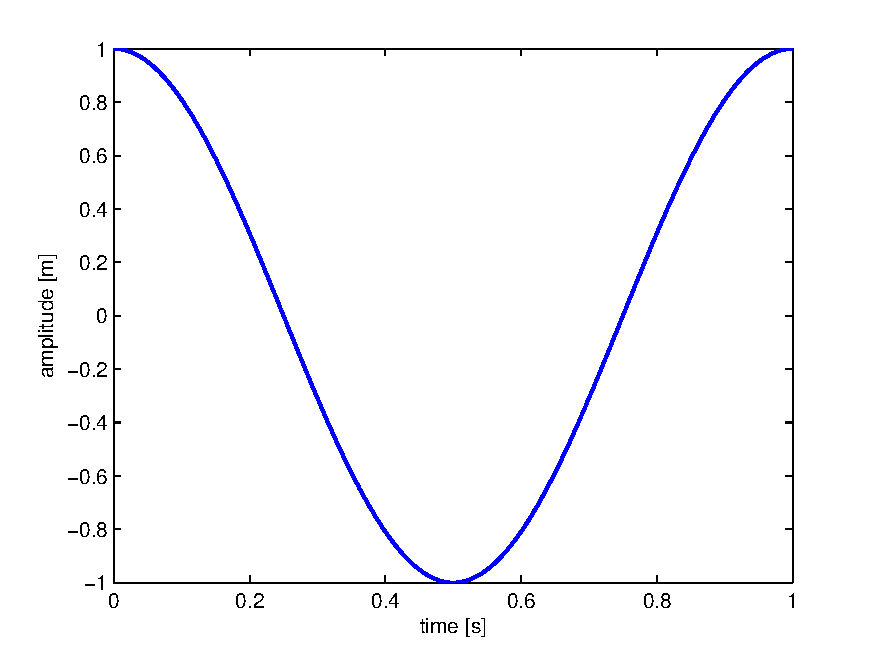
\includegraphics[width=\linewidth]{results}
	\caption{In-text Picture}
	\label{fig:results}
\end{figure}

Reference to Figure \ref{fig:results}.

%------------------------------------------------

\section{Results and Discussion}

\lipsum[10] % Dummy text

\subsection{Subsection}

\lipsum[11] % Dummy text

\begin{table}[hbt]
	\caption{Table of Grades}
	\centering
	\begin{tabular}{llr}
		\toprule
		\multicolumn{2}{c}{Name} \\
		\cmidrule(r){1-2}
		First name & Last Name & Grade \\
		\midrule
		John & Doe & $7.5$ \\
		Richard & Miles & $2$ \\
		\bottomrule
	\end{tabular}
	\label{tab:label}
\end{table}

\subsubsection{Subsubsection}

\lipsum[12] % Dummy text

\begin{description}
	\item[Word] Definition
	\item[Concept] Explanation
	\item[Idea] Text
\end{description}

\subsubsection{Subsubsection}

\lipsum[13] % Dummy text

\begin{itemize}[noitemsep] % [noitemsep] removes whitespace between the items for a compact look
	\item First item in a list
	\item Second item in a list
	\item Third item in a list
\end{itemize}

\subsubsection{Subsubsection}

\lipsum[14] % Dummy text

\subsection{Subsection}

\lipsum[15-23] % Dummy text

%------------------------------------------------

\phantomsection
\section*{Acknowledgments} % The \section*{} command stops section numbering

\addcontentsline{toc}{section}{Acknowledgments} % Adds this section to the table of contents

So long and thanks for all the fish \cite{Figueredo:2009dg, Smith:2012qr}.

%----------------------------------------------------------------------------------------
%	REFERENCE LIST
%----------------------------------------------------------------------------------------

\phantomsection
\bibliographystyle{unsrt}
\bibliography{bibliography.bib}

%----------------------------------------------------------------------------------------

\end{document}